%%%%%%%%%%%%%%%%%%%%%%%%%%%%%%%%%%%%%%%%%
% Friggeri Resume/CV
% XeLaTeX Template
% Version 1.1 (9/2/15)
%
% This template has been downloaded from:
% http://www.LaTeXTemplates.com
%
% Original author:
% Adrien Friggeri (adrien@friggeri.net)
% https://github.com/afriggeri/CV
%
% License:
% CC BY-NC-SA 3.0 (http://creativecommons.org/licenses/by-nc-sa/3.0/)
%
% Important notes:
% This template needs to be compiled with XeLaTeX and the bibliography, if used,
% needs to be compiled with biber rather than bibtex.
%
%%%%%%%%%%%%%%%%%%%%%%%%%%%%%%%%%%%%%%%%%
\documentclass[]{../friggeri-cv} % Add 'print' as an option into the square bracket to remove colors from this template for printing
\usepackage[danish]{babel}
\usepackage{icomma}
%\addbibresource{bibliography.bib} % Specify the bibliography file to include publications

\begin{document}

\header{morten emmanuel }{schiøler}{konsulent@deloitte consulting} % Your name and current job title/field

%----------------------------------------------------------------------------------------
%	SIDEBAR SECTION
%----------------------------------------------------------------------------------------

\begin{aside} % In the aside, each new line forces a line break
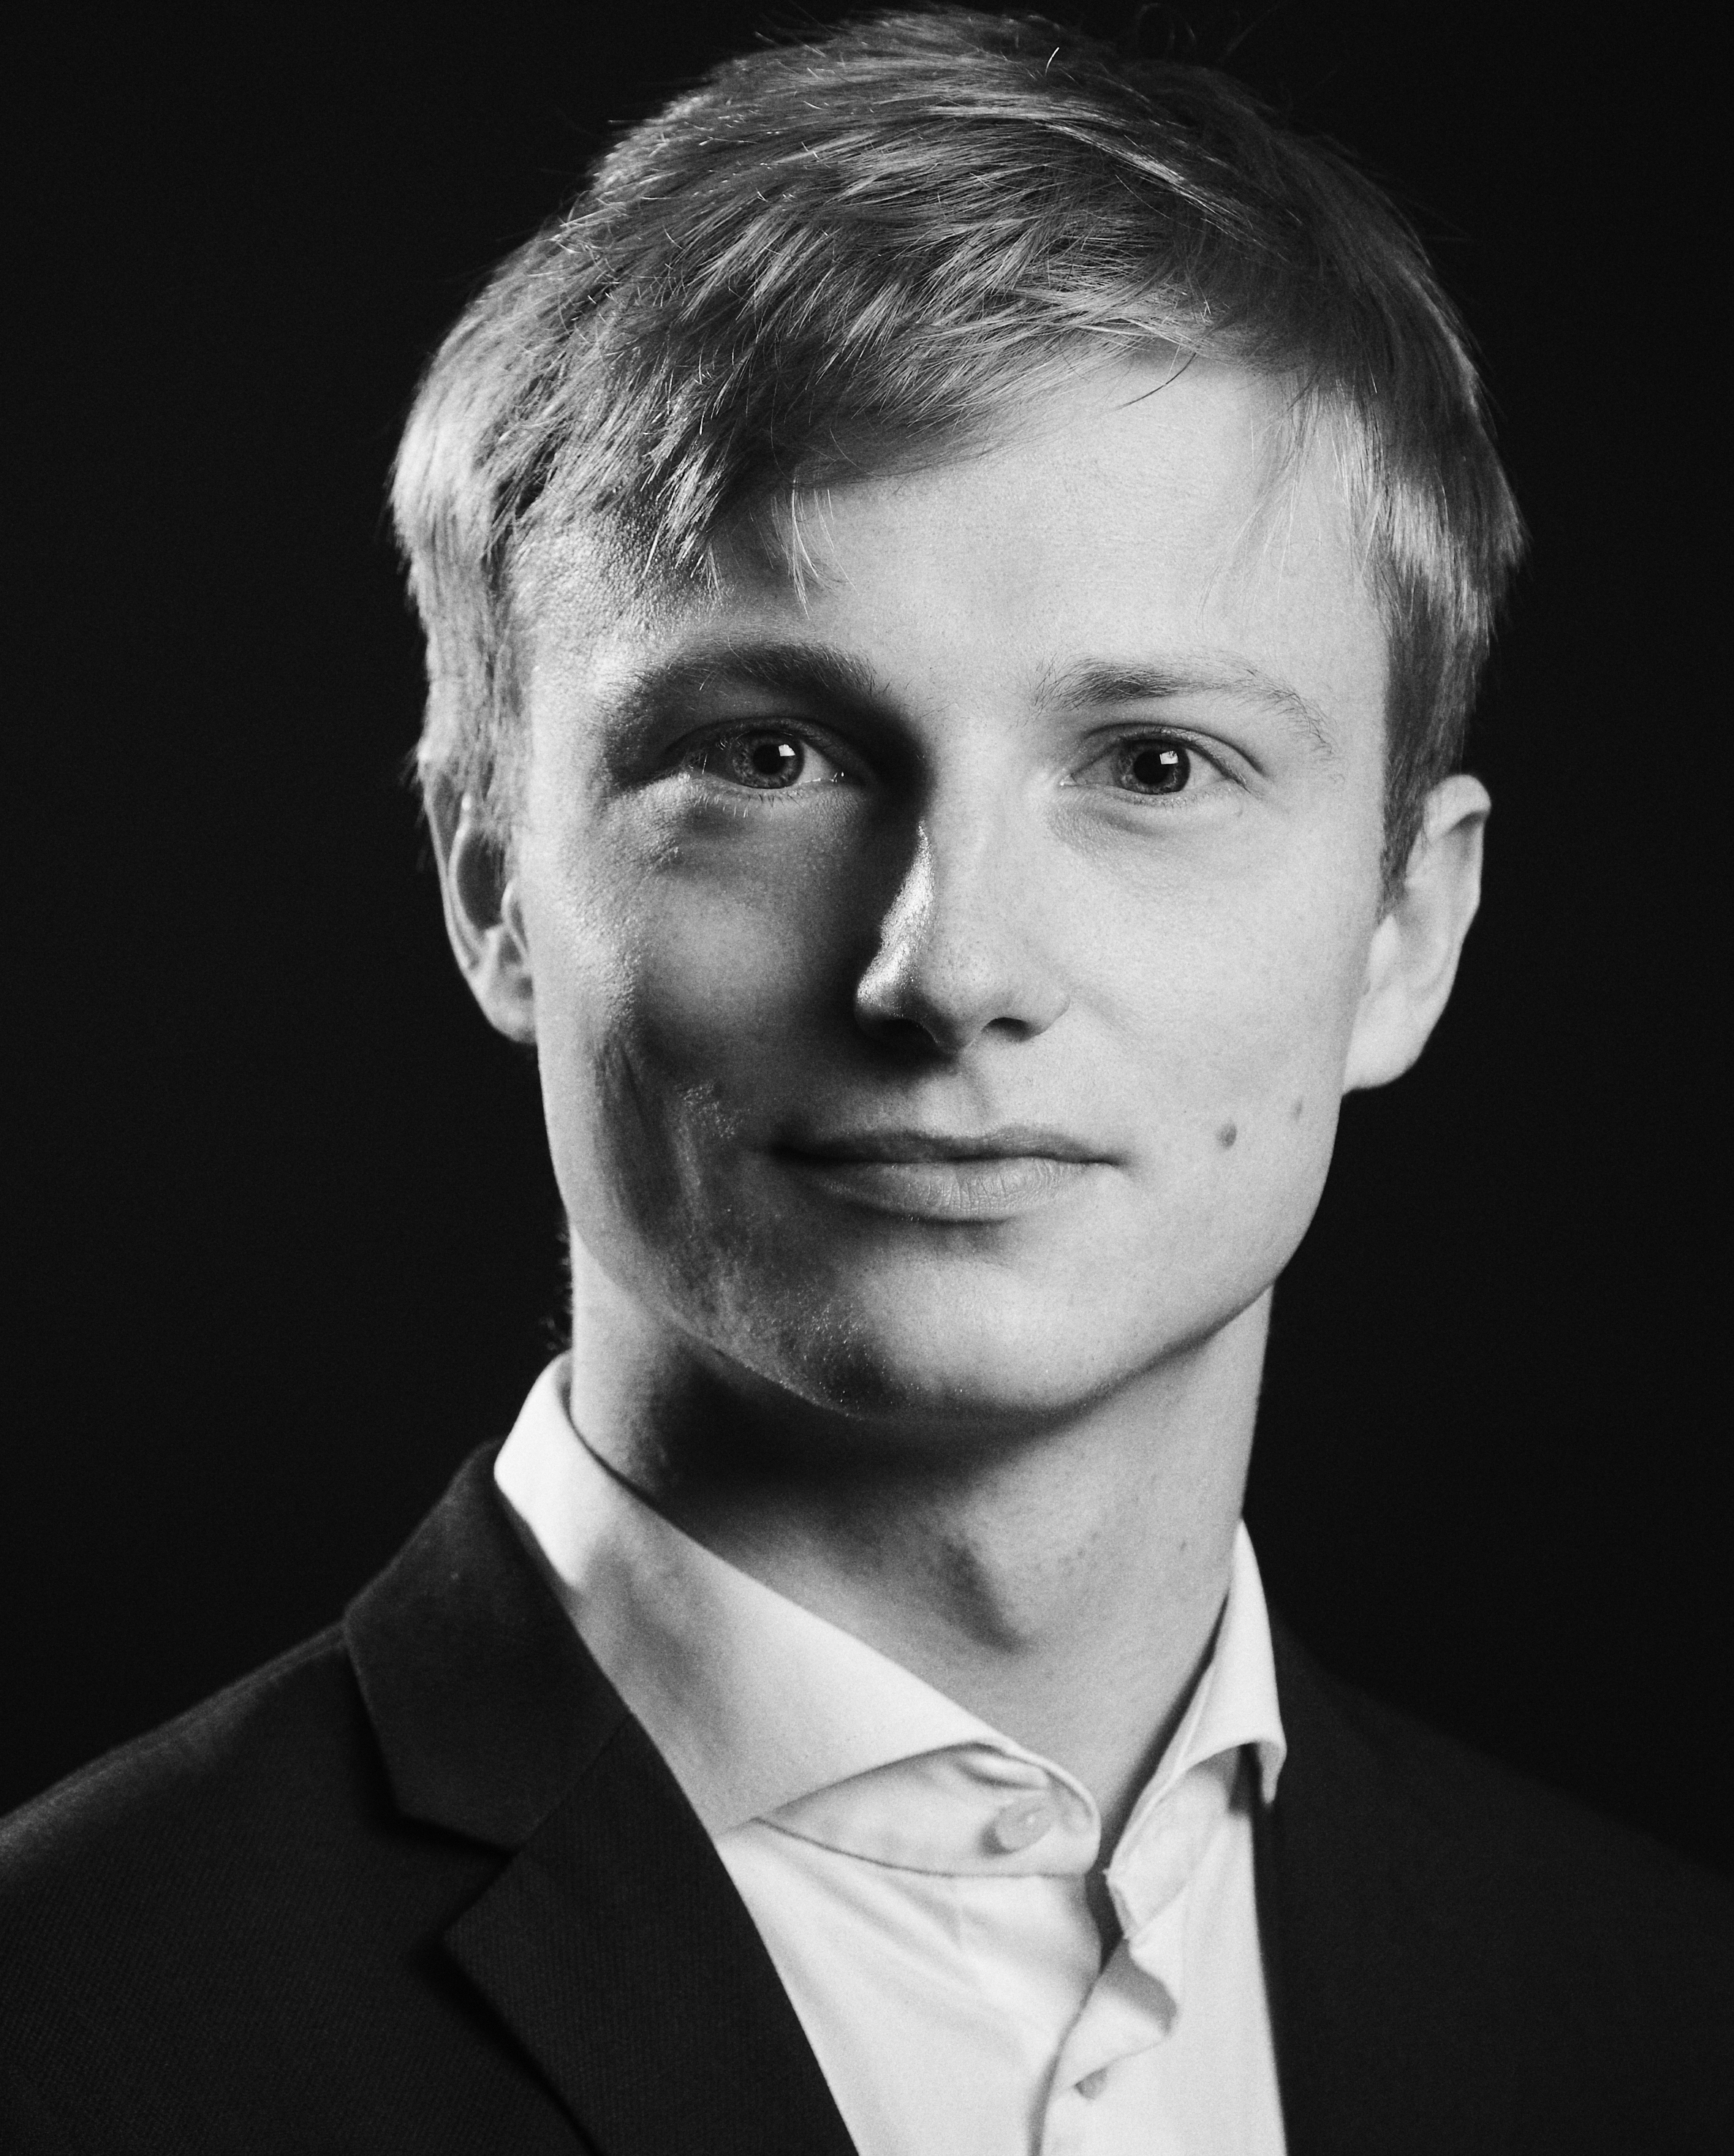
\includegraphics[width=\linewidth]{../graphics/pic8x10.jpg}
\section{kontakt}
Nordens Plads 12B,
1. sal, lejlighed nr.47
2000 Frederiksberg
~
+45 30 93 43 16
{\small \href{mschioeler@deloitte.dk}{mschioeler@deloitte.dk}}
\section{sprogkundskaber}
	dansk:  \quad modersmål
	engelsk: \quad flydende
	fransk: \quad begrænset praktisk færdighed
	rumænsk: \quad begrænset praktisk færdighed
%norwegian and swedish
\section{programmering}
{\color{red} $\varheartsuit$}Java \& Git 
Selenium, XPath
HTML, CSS, JavaScript
React.js
Flask \& Dash
REST
Ruby on Rails
UNIX/Bash
Python, \textsc{MATLAB}
SQL, SAS, R Statistics
RegExp
Lisp (Scheme)
%{\color{red} $\varheartsuit$} \LaTeX 
\end{aside}

%----------------------------------------------------------------------------------------
%	EDUCATION SECTION
%----------------------------------------------------------------------------------------
\section{profil}
En nysgærrig, lærenem og dreven konsultent med talent for- og tusindvis af timers erfaring i programmering. Elsker matematik og teknologi, er omhyggelig og ansvarsbevidst, og nyder samarbejde. 
\section{uddannelse}
\begin{entrylist}
%------------------------------------------------

\entry
{2014--2016}
{Kandidat {\normalfont i Transport og Logistik}}
{Danmarks Tekniske Universitet, Kgs. Lyngby}
{Omfattende studier i matematisk modellering, planlægning samt operationsanalyse, CBA og risikoanalyse. Tog kurser som f.eks. Optimering i Java, Heltalsprogrammering, Netværksoptimering og Risk Management. Afsluttet med et 12-tal (gennemsnit 11.25).
}

\entry
{2011--2014}
{Bachelor {\normalfont i Produktion og Konstruktion}}
{Danmarks Tekniske Universitet, Kgs. Lyngby}
{Bredt fagområde, bl.a.\ avanceret matematik og operationsanalyse, statistik og sandsynlighedsregning. Derudover fysik, styrkelære, procesteknik mv.}

%------------------------------------------------
%------------------------------------------------

\end{entrylist}

%----------------------------------------------------------------------------------------
%	COURSES SECTION
%----------------------------------------------------------------------------------------

\section{kurser}
\begin{entrylist}

%------------------------------------------------
%------------------------------------------------

\entry
{2017}
{Certified Kanban Management Professional}
{Deloitte, Weidekampsgade}
{Kursus i Kanbanteori og dets anvendelse i softwareudvikling.}

\entry
{2017}
{Leading SAFe (4.5)}
{Deloitte, Weidekampsgade}
{Officielt certifikat fra Scaled Agile Framework.}

\entry
{2017}
{Selvstudie {\normalfont i OOP}}
{}
{Gennemgik og implementerede størstedelen af design patterns fra \href{https://books.google.dk/books?id=6oHuKQe3TjQC}{Gang of Four} i Java.}


\entry
{2018}
{Selvstudie {\normalfont i Lisp}}
{}
{Implementerede en fungerende fortolker af Scheme Lisp, med REPL, i Python, på en eftermiddag.}

%------------------------------------------------
%------------------------------------------------
\end{entrylist}

%----------------------------------------------------------------------------------------
%	WORK EXPERIENCE SECTION
%----------------------------------------------------------------------------------------

\section{erfaring}

\subsection{deloitte consulting}

\begin{entrylist}
%------------------------------------------------
\entry
{2017--2018}
{IT-kompetencecenter for Inddrivelse (ICI)}
{Analytics \& Information Management @ DC}
{\emph{Testautomatiseringsekspert}\\
Udvikling af automatiserede browsertest af inddrivelsesløsningen PSRM. 
\begin{itemize}
\item Etablerede automatiseringsframework til browsertest ("ici-sel") baseret på Selenium i Java, som leverer en væsentlig forbedring i stabilitet, læsbarhed og brugervenlighed i forbindelse med automatisering for PSRM. 
\item Fungerede som teknisk ekspert i ici-sel og Java generelt. 
\item Administrerede Git-repository til automatiserede browsertests. 
\item Modtog præmie for at have faktureret næstflest timer (1374 i pågældende FY) i afdeling på tværs af WBS-numre på Skatteministeriets konto.
\end{itemize}
}

\end{entrylist}

\subsection{danmarks tekniske universitet}

\begin{entrylist}

\entry
{2016--2017}
{DTU Management}
{Danmarks Tekniske Universitet, Kgs. Lyngby}
{\emph{Videnskabelig assistent}\\
Adskillige akademiske opgaver, involverende modeludvikling, programmering, dataanalyse og grundforskning. Udførte avancereret dataanalyse i SAS og SQL.}

\entry
{2013--2015}
{DTU}
{Danmarks Tekniske Universitet, Kgs. Lyngby}
{\emph{Hjæperlærer}\\
Hjælpelærer i Heltalsprogrammering, Operationsanalyse og Fysik. Modtog skriftlig anbefaling for arbejde i operationsanalyse.}

\end{entrylist}


%----------------------------------------------------------------------------------------
%INTERESTS SECTION
%----------------------------------------------------------------------------------------
\section{interesser}
\textbf{professionelt:} softwaredesign og OOP, metaprogrammering, AI, matematisk modellering, statistik, operationsanalyse,  algoritmer, fysik
\textbf{personligt:} klaver, guitar, kaffe, sprog, spil
%----------------------------------------------------------------------------------------
%	PUBLICATIONS SECTION
%----------------------------------------------------------------------------------------
%
%\section{publications}
%
%\printbibsection{article}{article in peer-reviewed journal} % Print all articles from the bibliography
%
%\printbibsection{book}{books} % Print all books from the bibliography
%
%\begin{refsection} % This is a custom heading for those references marked as "inproceedings" but not containing "keyword=france"
%\nocite{*}
%\printbibliography[sorting=chronological, type=inproceedings, title={international peer-reviewed conferences/proceedings}, notkeyword={france}, heading=subbibliography]
%\end{refsection}
%
%\begin{refsection} % This is a custom heading for those references marked as "inproceedings" and containing "keyword=france"
%\nocite{*}
%\printbibliography[sorting=chronological, type=inproceedings, title={local peer-reviewed conferences/proceedings}, keyword={france}, heading=subbibliography]
%\end{refsection}
%
%\printbibsection{misc}{other publications} % Print all miscellaneous entries from the bibliography
%
%\printbibsection{report}{research reports} % Print all research reports from the bibliography
%
%----------------------------------------------------------------------------------------
%
\end{document}
